\documentclass{beamer}
%
% Choose how your presentation looks.
%
% For more themes, color themes and font themes, see:
% http://deic.uab.es/~iblanes/beamer_gallery/index_by_theme.html
%
\mode<presentation>
{
    \usetheme{default}      % or try Darmstadt, Madrid, Warsaw, ...
    \usecolortheme{default} % or try albatross, beaver, crane, ...
    \usefonttheme{default}  % or try serif, structurebold, ...
    \setbeamertemplate{navigation symbols}{}
    \setbeamertemplate{caption}[numbered]
}

\usepackage[english]{babel}
\usepackage[utf8]{inputenc}
\usepackage[T1]{fontenc}
\usepackage{graphicx}
\usepackage{hyperref}

\title[Your Short Title]{Project Presentation}
\author{Alessandro Lombardi}
\institute{Artificial Intelligence - University of Bologna}
\date{08-05-2020}

\begin{document}

\begin{frame}
    \titlepage
\end{frame}

% Uncomment these lines for an automatically generated outline.
%\begin{frame}{Outline}
%  \tableofcontents
%\end{frame}

\section{Introduction}\label{sec:introduction}

\begin{frame}{Introduction}

    \begin{block}{The idea}
    Analyze Ethereum Blockchain as a network of transactions between addresses.
    \end{block}

    \vskip 1cm

    \begin{block}{The Ethereum Blockchain}
        Some stats to get an idea of the involved numbers
        \begin{itemize}
            \item latest \textbf{block} height value higher than 10 million
            \item more than 96 million unique \textbf{addresses}
            \item more than 698 million \textbf{transactions}
            \item Ethereum blocks are mined every 20 seconds
        \end{itemize}
        Source: \url{https://etherscan.io/}
    \end{block}

\end{frame}

\begin{frame}{}
    \begin{figure}
        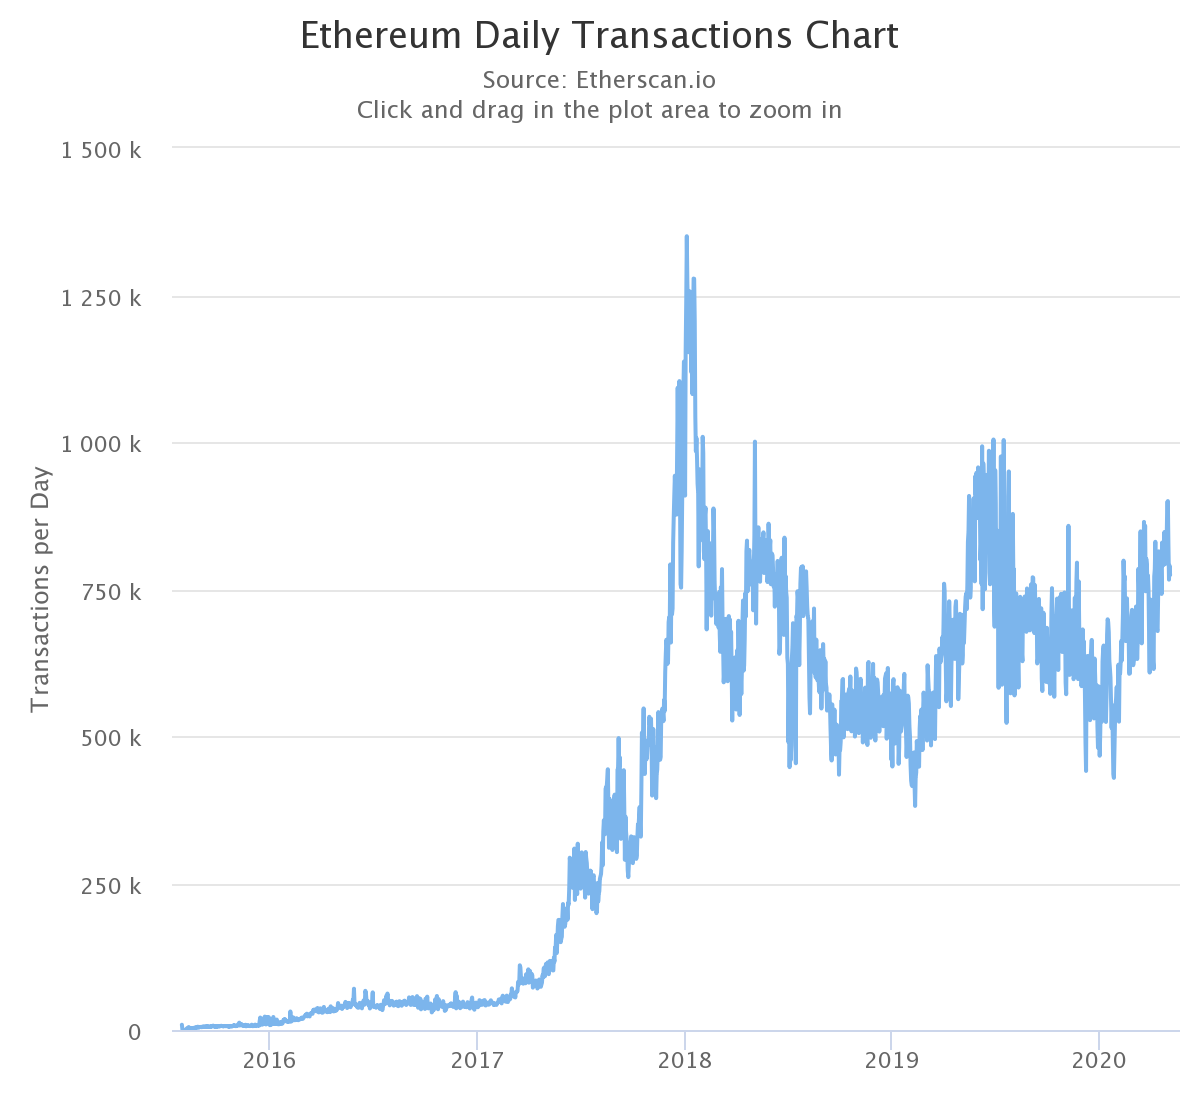
\includegraphics[scale=0.235]{daily_txs_chart.png}
        \caption{}\label{fig:figure}
    \end{figure}
\end{frame}

\begin{frame}{Addresses}
    \begin{block}{}
        In Ethereum and Solidity, an address is a 20 byte (160 bits or 40 hex characters) alphanumeric string.
        It corresponds to the last 20 bytes of the Keccak-256 hash of the public key.
    \end{block}

    \begin{figure}
        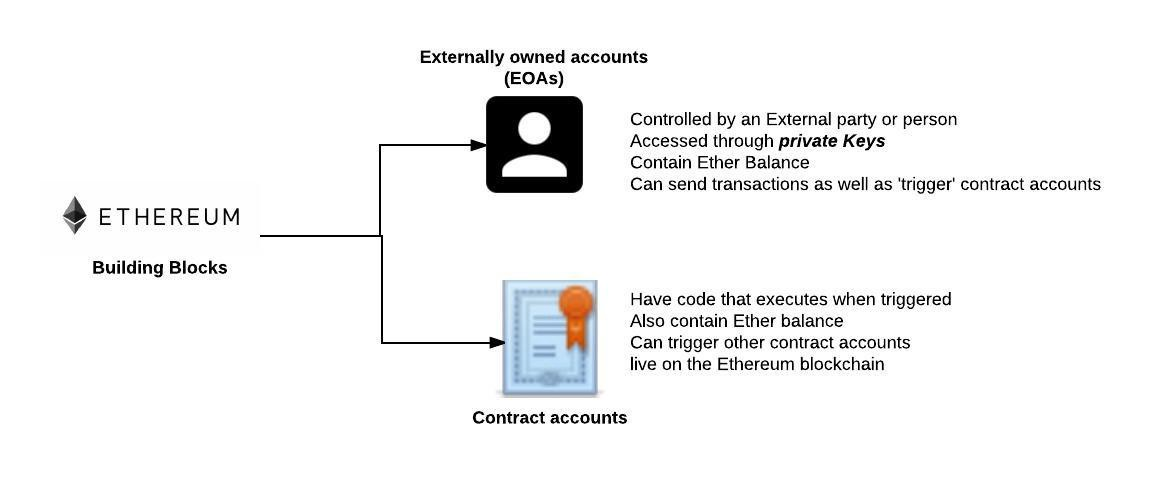
\includegraphics[width=\textwidth]{types_of_addresses.jpeg}
        \caption{Source: \href{https://hackernoon.com/heres-how-i-built-a-private-blockchain-network-and-you-can-too-62ca7db556c0}{Abhishek Chakravarty, Hackernoon.com}}\label{fig:figure2}
    \end{figure}

\end{frame}

\begin{frame}{Transactions}
    \begin{block}{}
        While transactions are used for different purposes, the transaction structure is the same.
        The amount of fund is expressed in wei (1 ether = $10^{18}$ weis).
        Contracts can receive transfers just like externally controlled accounts, but they can also receive more complicated transactions that actually run parts of their code and update their state.
    \end{block}

    \vskip 0.75cm

    \begin{block}{Types}
        \begin{itemize}
            \item \textbf{Fund Transfer Between EOA} used when an EOA is transferring fund to another EOA\@.
            \item \textbf{Deploy a Contract on Ethereum Network} used to deploy a compiled contract
            \item \textbf{Execute a Function on a Deployed Contract}
        \end{itemize}
    \end{block}
\end{frame}

\begin{frame}{Clustering coefficients}
    \begin{block}{}
        Graph $(V,E)$ without self loops and multiple edges.
    \end{block}

    \vskip 0.5cm

    \begin{block}{Transitivity}
        The fraction of all possible triangles (closed triplets) present in G. Possible triangles are identified by the number of “triads” (two edges with a shared vertex, open and closed triplets): $3\cfrac{|triangles|}{|triads|}$
    \end{block}

    \begin{block}{Global clustering coefficient}
        The sum of fractions of number of triangles over number of open or closed triples passing on each vertex with degree greater than 2 (called $N_2$):
        $\cfrac{1}{N_2} \sum_{i \in V, d_i \geq 2}\cfrac{|triangles per vertex|}{|triads per vertex|}$
    \end{block}
\end{frame}

\begin{frame}

    \begin{block}{Local clustering coefficient}
        Quantifies how close the neighbours of a vertex in a graph are to being a clique (complete graph): $\cfrac{|\{e_{jk} : v_j, v_k \in N_i, e_{jk} \in E\}|}{|N_i|(|N_i| - 1)}$
    \end{block}

    \begin{block}{}
        Where $E$ is the set of edges and $V$ the set of vertices. $N_i$ is the set of neighbors of the $i^{th}$ node.
    \end{block}

\end{frame}

\begin{frame}{Modularity}
    \begin{block}{}
        Measure the strength of division of a network into modules (also called groups, clusters or communities).
        Networks with high modularity have dense connections between the nodes within modules but sparse connections between nodes in different modules.
    \end{block}
    \begin{block}{}
        $\sum_{i=1}^{c}(e_{ii} - a_{i}^{2})$, where $e_{ij} = \cfrac{edges from i to j}{2|E|}$ and $a_i = \cfrac{k_i}{2|E|}$
    \end{block}

    \begin{block}{}
        Fraction of edges that fall within communities, minus the expected value of the same quantity if edges fall at random without regard for the community structure, which is the total degree of the cluster.
    \end{block}
\end{frame}

\begin{frame}{Community Detection}
    \begin{block}{Two different concepts}
        \begin{itemize}
            \item Clustering
            \item Partitioning
        \end{itemize}
    \end{block}
    \begin{block}{Clustering methods}
        \begin{itemize}
            \item Label Propagation
            \item Louvain Method
            \item Minimum Cut Three
            \item Dynamic Clustering
        \end{itemize}
    \end{block}

\end{frame}

\begin{frame}{Further works}
    \begin{block}{Deanonymize the network}
        Add more features to addresses, scraping from the web (forums, datasets etc..).
    \end{block}

    \vskip 1cm

    \begin{block}{Cluster users}
        Adopt Machine Learning/Data Mining techniques to cluster addresses based on activity (Miners, ICO, etc..) in addition to topology.
    \end{block}
\end{frame}

\end{document}
